\documentclass[a4paper,12pt]{article}
\usepackage[left=2cm, right=2cm, top=2cm]{geometry}
\usepackage{graphicx} 
\usepackage[export]{adjustbox}
\usepackage{titlepic}
\usepackage{amssymb}
\usepackage{titling}
\usepackage[utf8]{inputenc}
\usepackage{listings}
\usepackage{color}
\usepackage[T1]{fontenc}
\usepackage[utf8]{inputenc}
\usepackage{wrapfig}
\usepackage{helvet}
\usepackage{fourier} 
\usepackage{array}
\usepackage{makecell}
%\usepackage[square,sort,comma,numbers]{natbib}
\usepackage{ragged2e}
\usepackage{placeins}
\bibliographystyle{IEEEtran}
\usepackage{float}
\setlength{\belowcaptionskip}{-15pt}
\renewcommand{\familydefault}{\sfdefault}
\newcommand{\squeezeup}{\vspace{-2.5mm}}
\definecolor{codegreen}{rgb}{0,0.6,0}
\definecolor{codegray}{rgb}{0.5,0.5,0.5}
\definecolor{codepurple}{rgb}{0.58,0,0.82}
\definecolor{backcolour}{rgb}{0.95,0.95,0.92}

\renewcommand\theadalign{bc}
\renewcommand\theadfont{\bfseries}
\renewcommand\theadgape{\Gape[4pt]}
\renewcommand\cellgape{\Gape[4pt]}

\usepackage{fancyhdr,lipsum}
\pagestyle{fancy}
\fancyhf{}% Clear header/footer

\usepackage{hyperref}
\hypersetup{
    colorlinks,
    %citecolor=gray,
    citecolor=black,
    filecolor=black,
    linkcolor=black,
    urlcolor=black,
    linktoc=all
}

\lstdefinestyle{mystyle}{
    backgroundcolor=\color{backcolour},   
    commentstyle=\color{codegreen},
    keywordstyle=\color{blue},
    numberstyle=\tiny\color{codegray},
    stringstyle=\color{codepurple},
    basicstyle=\tiny,
    breakatwhitespace=false,         
    breaklines=true,                 
    captionpos=b,                    
    keepspaces=true,                 
    numbers=left,                    
    numbersep=5pt,                  
    showspaces=false,                
    showstringspaces=false,
    showtabs=false,                  
    tabsize=2
}


\chead{%
  \ifcase\value{page}
  % empty test for page = 0
  \or % page=1
  \or % page = 2
  \or Alexander Bolton% page = 3
  \or Author% page = 4
  \or Author% page = 5
  \or Author% page = 6
  \or Author% page = 7
  \or Author% page = 8
  \or Author% page = 9
  \or Author% page = 10
  \or Author% page = 11
  \or Author% page = 12
  \or Author% page = 13
  \or % page = 14
  \else
  % Empty chead here!
  \fi
}

\cfoot{\thepage}

\lstset{style=mystyle}

\pretitle{%
  \begin{center}
  \LARGE

\includegraphics[width=0.5\textwidth, right]{UniLogo.png}\\[\bigskipamount]

\hspace{15cm}

\hspace{27cm}

\hspace{27cm}

\hspace{10cm}
}
\posttitle{\end{center}}	

\begin{document}

\title{\\ \textbf{ELEC5620M \\ Mini Project \\ \- \\ DE1-SoC Pong }}
\author{Alexander Bolton - 200938078 \\ Sam Wilcock - 201285260\\ John Jakobsen - }
\date{May 2019}
\maketitle
\begin{center}
Submitted in accordance with the requirements for the degree of \\
Master of Science in Embedded Systems Engineering
\end{center}
\vfill
\begin{center}
The University of Leeds \\  School of Electronic and Electrical Engineering
\end{center}
\newpage

\tableofcontents
\newpage 
\section{Introduction}
\begin{flushleft}
This report will discuss the group project for the Embedded Microprocessor System Design module. The groups member's were Alexander Bolton, Sam Wilcock, and John Jakobsen. The projects aim was to create a game of Pong on the DE1-SoC's microprocessor unit (MPU) which utilised the LT24 LCD Screen, a VGA screen, PS2 keyboard controls, button controls, and have audio output.
\\ \- \\
This report will be broken down into sections with section 1 being the introduction. Section 2 will discuss the display and graphics side of the project including the VGA driver which controls the monitor, the display driver which controls both LCD and VGA screens with a frame buffer, sprites and text which will go into depth of how the sprites are created, finally game engine graphics which will go into how the game engine uses the sprites including destroying, creating, and moving the sprites. 
\\ \- \\
Section 3 will discuss...
\\ \- \\
Section 4 will discuss...
\\ \- \\
Section 5 will be the conclusion which will summarise the report and discuss if we have met the aims of the project. It will discuss what could be improved upon and changed. All code will be placed in the end of the report in the appendices. 
\end{flushleft}
\newpage
\section{Display and Graphics}
\subsection{VGA Driver}
\begin{flushleft}
This subsection discusses the VGA driver and how it was implemented in the project. The VGA video out supports 640x480 however in this project is set to the default value of 320x240 pixels. The image displays from the VGA controller which is addressed from a pixel buffer. Each pixel value is addressable using equation 1. An example of the pixel at 0,1 is shown in equation 2. The default base address for the pixel buffer is 0xC8000000 as stated in the manual. \cite{altera_2014} 
\begin{equation}
	VGA_{base address} + (pixelX_{coordinates}\:pixelY_{coordinates}\:0_{2})
\end{equation}
\begin{equation}
	C8000000_{16} + (00000001\:000000000\:0)_{2} = C8000400_{16}
\end{equation}
The pixels are layed out with the y coordinate starting from the top to bottom of the screen. The x coordinate is from right to left of the screen as shown in figure 1.
\begin{figure}[H]
	\centering
	\fbox{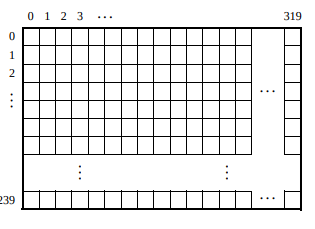
\includegraphics[width=0.4\textwidth]{./images/VGAPixels.png}}
	\caption{Pixel layout for pixel buffer of VGA controller \cite{altera_2014}}
\end{figure}
\- \\
Each pixel once addressed can be set to a value of colour with by setting bits for red, green, and blue. Each colour is allocated 5 bits which indicate the strength of colour for the pixel as shown in figure 2. 
\begin{figure}[H]
	\centering
	\fbox{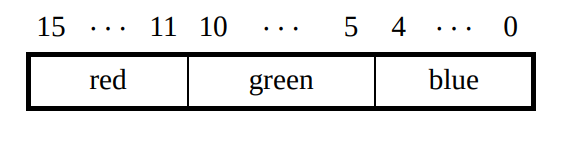
\includegraphics[width=0.3\textwidth]{./images/VGAPixelcolour.png}}
	\caption{Pixel Colour Layout \cite{altera_2014}}
\end{figure}
\- \\
This code extracted from the project shows how a pixel is set in C.
\begin{figure}[H]
	\centering
	\lstinputlisting[language=C, firstline=20, lastline=25, frame=bt]{../DE1_SOC_PONG/DE1SoC_VGA/DE1SoC_VGA.c}
		\caption{Code used to set pixel to a colour.}
\end{figure}
\end{flushleft}
\newpage
\subsection{Display Driver}
\begin{flushleft}
•
\end{flushleft}
\newpage
\subsection{Sprites and Text}
\begin{flushleft}
•
\end{flushleft}
\newpage
\subsection{Game Engine Graphics}
\begin{flushleft}
•
\end{flushleft}
\newpage
\section{Controls and Menus}
\newpage
\section{Game Physics}
\newpage
\section{Conclusion}
\begin{flushleft}

\end{flushleft}
\newpage
\section{Appendix}
\newpage
\addcontentsline{toc}{section}{References}
\begin{flushleft}
\bibliography{refs}
\end{flushleft}
\end{document}
